%%%%%%%%%%%%%%%%%%%%%%%%%%%%%%%%%%%%%%%%%
% Friggeri Resume/CV
% XeLaTeX Template
% Version 1.2 (3/5/15)
%
% This template has been downloaded from:
% http://www.LaTeXTemplates.com
%
% Original author:
% Adrien Friggeri (adrien@friggeri.net)
% https://github.com/afriggeri/CV
%
% License:
% CC BY-NC-SA 3.0 (http://creativecommons.org/licenses/by-nc-sa/3.0/)
%
% Important notes:
% This template needs to be compiled with XeLaTeX and the bibliography, if used,
% needs to be compiled with biber rather than bibtex.
%
%%%%%%%%%%%%%%%%%%%%%%%%%%%%%%%%%%%%%%%%%

\documentclass[]{friggeri-cv} % Add 'print' as an option into the square bracket to remove colors from this template for printing

\addbibresource{bibliography/publications.bib} % Specify the bibliography file to include publications

\begin{document}


\header{Malcolm}{Ramsay}{Honours Student} % Your name and current job title/field

%----------------------------------------------------------------------------------------
%	SIDEBAR SECTION
%----------------------------------------------------------------------------------------

\begin{aside} % In the aside, each new line forces a line break
    \vspace{30 mm}~
\begin{flushleft}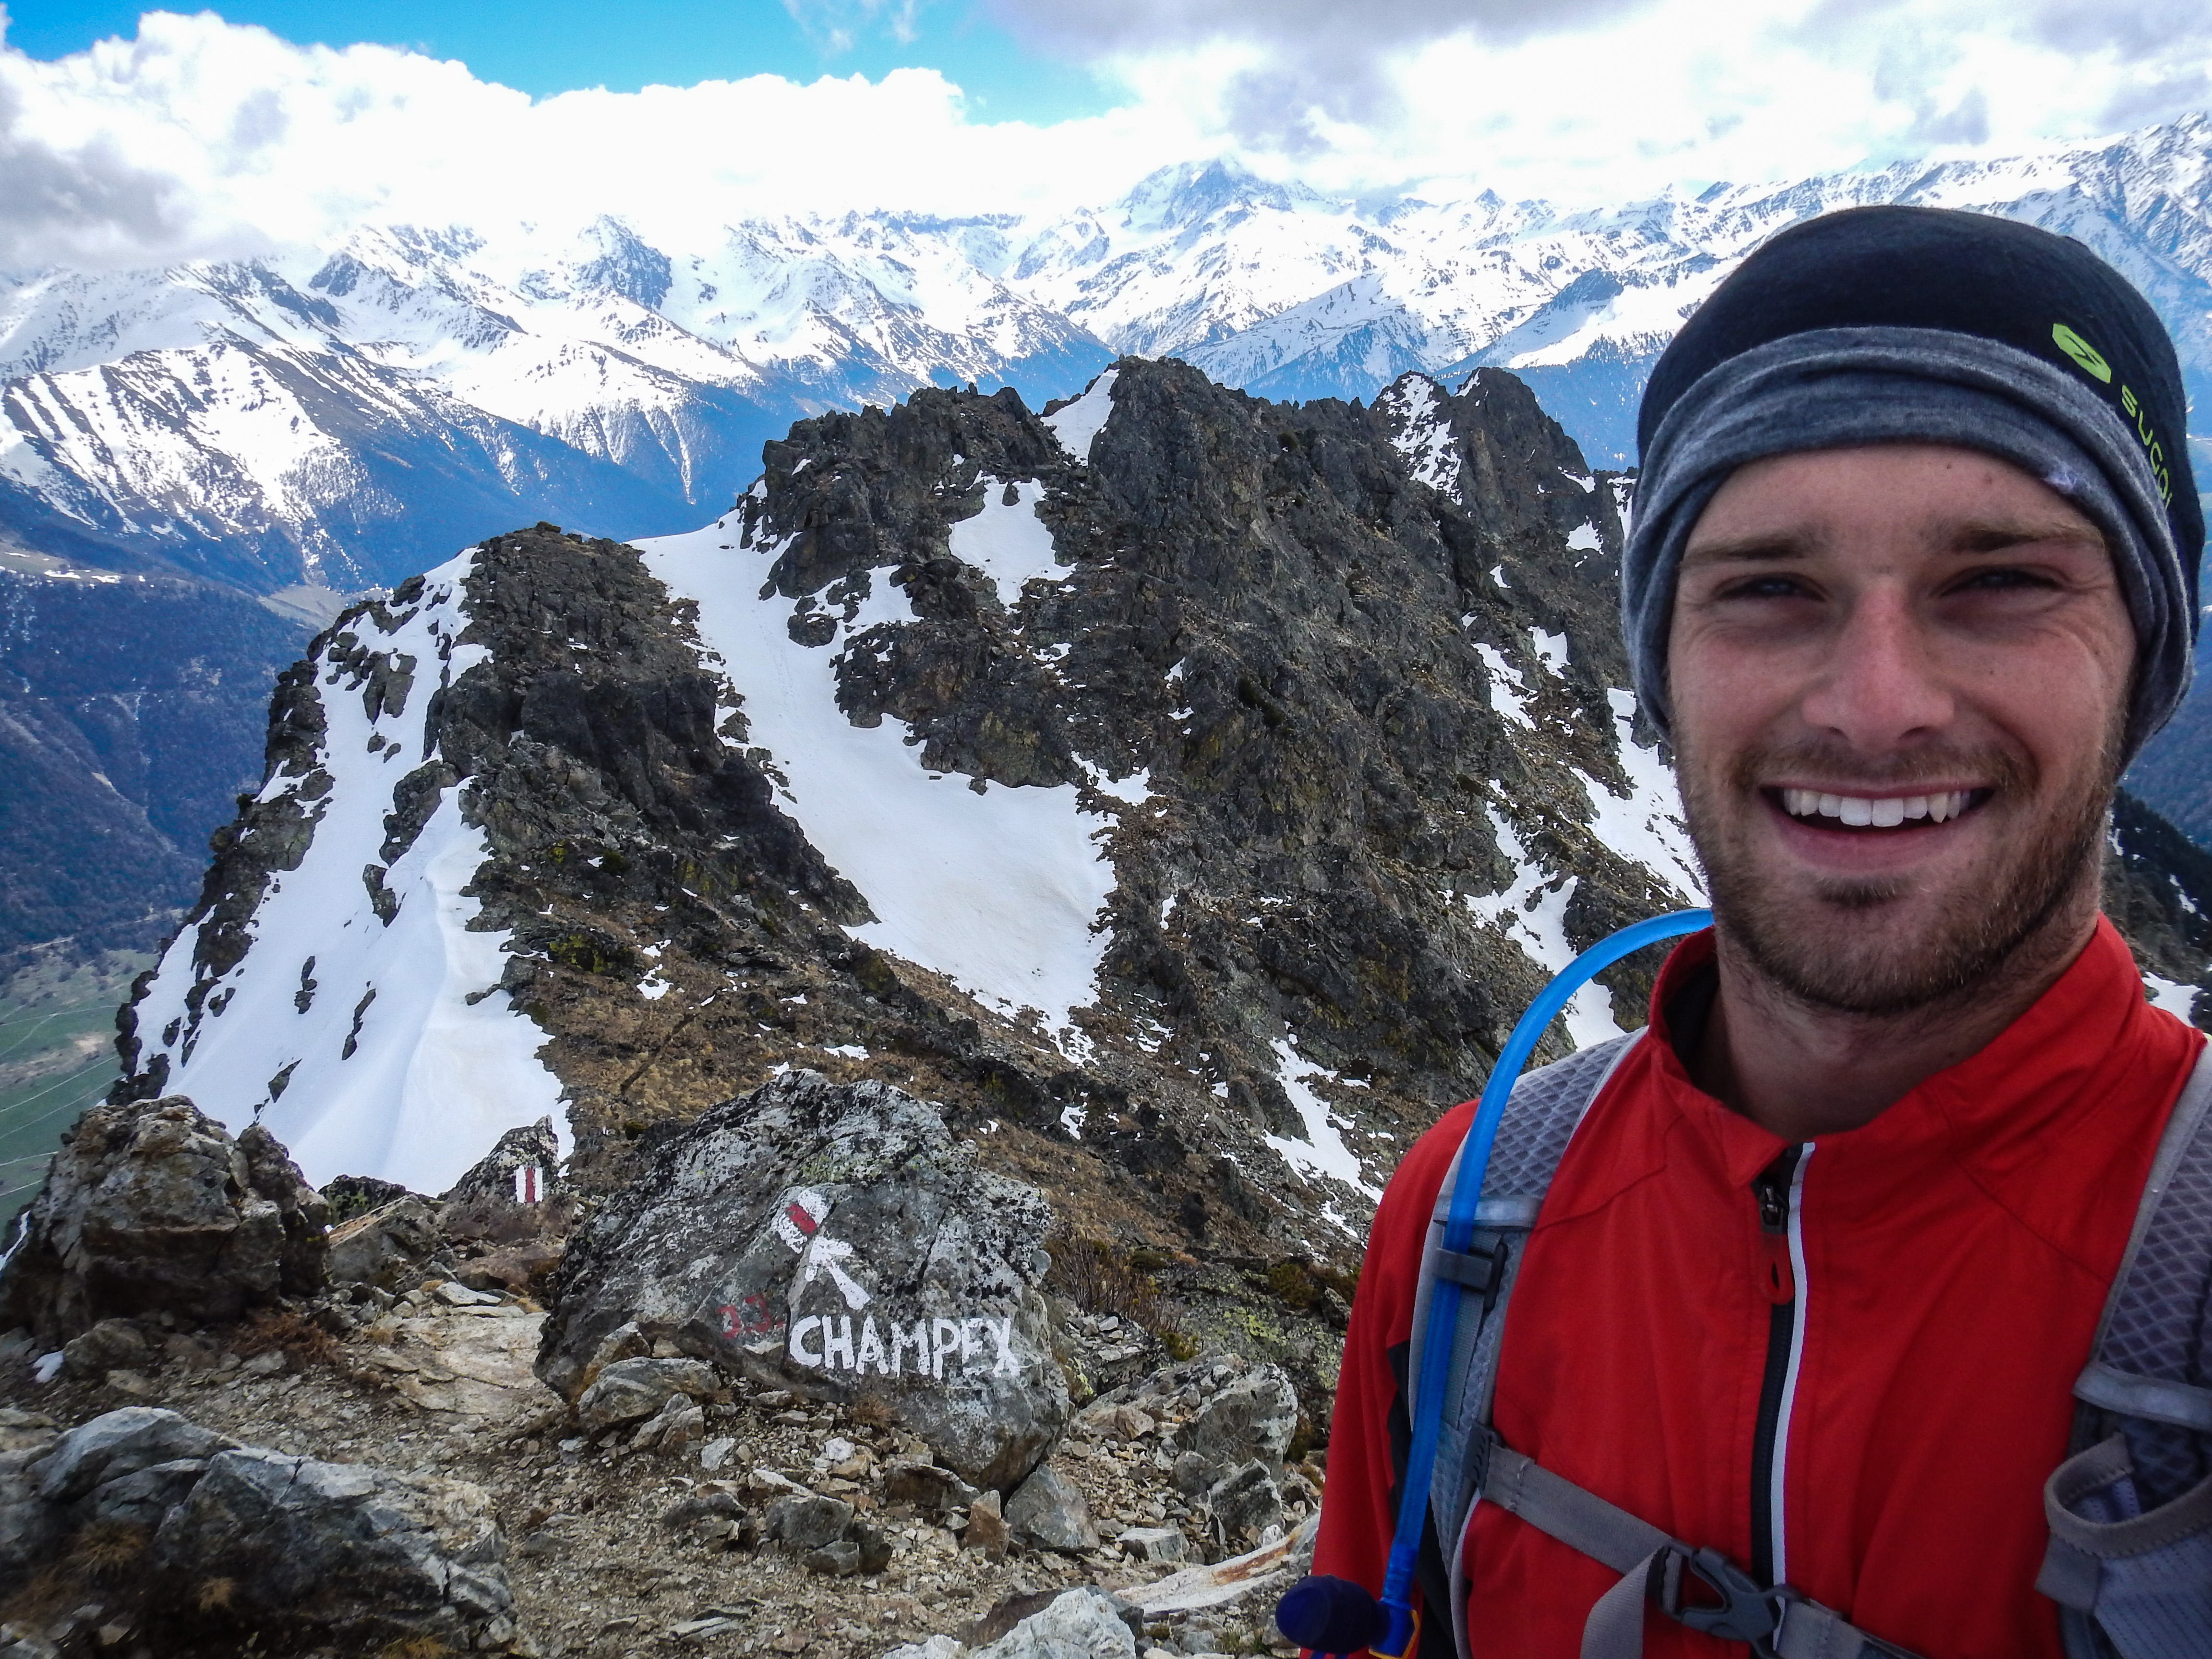
\includegraphics[width=3.6em]{portrait}\\\end{flushleft}~
\section{Contact}
0466 224 898
\href{mailto:malramsay64@gmail.com}{malramsay64@gmail.com}
\section{Programming}
Python, C++, C, Bash,
Matlab, Mathematica,
\LaTeX, Fortran, Git,
Unix, Make, MPI
\end{aside}

%----------------------------------------------------------------------------------------
%	EDUCATION SECTION
%----------------------------------------------------------------------------------------

\section{Education}

\begin{entrylist}

%------------------------------------------------

\entry
{2009--2015}
{Bachelor of Science (Advanced) Honours}
{University of Sydney}
{\emph{The Role of Molecular Shape on the Properties of the Condense Phase: A Simulation Study}
}

%------------------------------------------------

\entry
{2013--2014}
{Exchange Semester}
{The University of California, Santa Barbara}
{I undertook an academic exchange in the final semester of my degree. I received both the Dean of Science Undergraduate Exchange Scholarship and an International Exchange Scholarship from the University of Sydney in support of my exchange.}

%------------------------------------------------

\entry
{2009}
{Chemistry Olympiad Summer School}
{}
{After spending two weeks at Monash University learning most 1st year and some 2nd year Chemistry I placed 11th in the Australian Chemistry Olympiad, competing against the top high school chemistry students in Australia.}

\entry
{2004--2009}
{Higher School Certificate}
{Normanhurst Boys High School}
{In my final year at school I was awarded Senior Sportsman of the year, CALTEX All-rounder award, Buttfield Memorial Trophy for best and fairest in Open Soccer, Best and Fairest in 1st Grade Waterpolo, and I was a Sydney North Area Representative in Athletics and Cross Country. I was Age Champion in Swimming, Cross Country and Athletics for all of my six years at High School. My ATAR was 95.75.
}


\end{entrylist}


%----------------------------------------------------------------------------------------
%	PUBLICATIONS SECTION
%----------------------------------------------------------------------------------------

\section{Publications}

\printbibsection{article}{Articles} % Print all articles from the bibliography

%----------------------------------------------------------------------------------------
%	WORK EXPERIENCE SECTION
%----------------------------------------------------------------------------------------

\section{Experience}

\subsection{Full Time}

\begin{entrylist}

%------------------------------------------------

\entry
{2012}
{Australian Sports Drug Testing Laboratory}
{National Measurement Institute}
{\emph{Year in Industry Student} \\
 was a Year in Industry student at ASDTL partaking in two main research projects. One involving the detection of peptides in urine utilising Nanoflow Electrospray Liquid Chromatography coupled with an Orbitrap Mass Spectrometer. I was responsible for calibration and routine maintenance of this instrument. I was also involved with testing the idea of machine learning tools to flag samples as anomalous despite not directly identifying a compound of interest.}

%------------------------------------------------

\end{entrylist}

\subsection{Part Time}

\begin{entrylist}

\entry
{2010--2015}
{1/15 RNSWL Band}
{Australian Army Reserves}
{\emph{Musician} \\
s a musician I am required to be part of the public face of the Army, performing with the unit band at a number of military events, such as ANZAC day, Reserve Forces Day and any other events that are tasked to the band. In being part of the public face of the Army I am required to adhere to the standards of dress and bearing, upholding the expectations of the public.

As part of the band I am also required to provide entertainment for Army functions, primarily dining in nights and end of year celebrations.

As a bugler I am required as an individual to perform bugle calls at ceremonial functions.

Viral video
}

%------------------------------------------------

\entry
{2014--2015}
{School of Chemistry}
{University of Sydney}
{\emph{1\textsuperscript{st} Year Demonstrator} \\

}

%------------------------------------------------

\entry
{2011}
{Summer Scholarship}
{School of Chemistry, University of Sydney}
{
}


\entry
{2009--2013}
{Trumpet Tutor}
{}
{I have tutored several students towards their AMEB practical and theory exams. I give them lessons each week, and teach them the skills required to pass their theory and practical exams. I have had a number of students receive music scholarships at private schools.}

\entry
{2004--2012}
{Football (Soccer) Referee}
{Gladesville Horsby Football Referees Association}
{I was a member of Gladesville Hornsby Football Association. I mentored and assessed junior referees to assist in their development as referees. This required me to attend their games and provide constructive feedback, reporting back to the technical committee of the association. I was also a member of the Elite Development Program to challenge and develop promising referees, providing opportunities to officiate the highest divisions of youth football in NSW.
}

\end{entrylist}

%----------------------------------------------------------------------------------------
%	AWARDS SECTION
%----------------------------------------------------------------------------------------

\section{Awards}

\begin{entrylist}

%------------------------------------------------

\entry
{2015}
{Walter Moore Scholarship}
{School of Chemistry, University of Sydney}
{
}

\entry
{2013}
{Dean of Science Undergraduate Exchange Scholarship}
{School of Chemistry, University of Sydney}
{
}

\entry
{2013}
{International Exchange Scholarship}
{International Office, University of Sydney}
{
}

\entry
{2009}
{Levy Scholarship}
{School of Chemistry, University of Sydney}
{
}

%------------------------------------------------

\end{entrylist}

%----------------------------------------------------------------------------------------
%	EXTRA CURRICULAR
%----------------------------------------------------------------------------------------

\section{Extra Curricular Activities}

\begin{entrylist}

%------------------------------------------------

\entry
{2012--Present}
{Triathlon}
{}
{
}

\entry
{2009--2014}
{Science Revue}
{}
{
}

\entry
{2010--2013}
{Millennium Marching Band Tutor}
{Department of Education and Communities}
{I volunteered as a tutor with the Millennium Marching Band, I was in charge of warming up the band physically for a whole day rehearsal on the field. This included stretching and fun games. I also assisted with the trumpet section providing musical guidance and assisting students learn music.}

\entry
{2010--2011}
{National Computer Science School Challenge Tutor}
{}
{The NCSS Challenge is a programming competition for school students from years 5 to 12. There are varying levels of questions for differing abilities. As a tutor I responded to questions from the students mainly directed at issues they were having on the problems for that week but also general programing questions. Also involved was encouraging students to have fun programming and encourage learning after the completion of the competition.}

\entry
{2009}
{School Prefect}
{Normanhurst Boys High School}
{I was a prefect at high school which involved me running fundraising events such as barbeques and mufti days and being part of the public face of the school.}

\entry
{2008}
{Beijing Olympic Orchestra}
{}
{In 2008 I was part of the NSW contingent that went over to Beijing as part of the 2000 piece Olympic Orchestra. We performed in such places as the Great Wall, we were the first western group to perform in Tiananmen Square and we performed before the first event of the Olympics, the women's football in Tian Jing}

%------------------------------------------------

\end{entrylist}

%----------------------------------------------------------------------------------------
%	INTERESTS SECTION
%----------------------------------------------------------------------------------------

\section{Hobbies}

\begin{entrylist}

\entry
{}
{Photography}
{}
{Photographing USU Events}

\entry
{}
{Music}
{}
{NWWE National Championships}

\end{entrylist}

%----------------------------------------------------------------------------------------

\end{document}
